%!TEX program = xelatex
\documentclass[a4paper]{article}

\usepackage[dvipsnames]{xcolor}

\usepackage{fancyhdr}
\usepackage{extramarks}
\usepackage{amsmath}
\usepackage{amsthm}
\usepackage{amsfonts}
\usepackage{tikz}
\usepackage[plain]{algorithm}
\usepackage{algpseudocode}

\usepackage{ctex}
\usepackage{indentfirst}
\usetikzlibrary{automata,positioning,shapes.geometric,arrows.meta,patterns,calc}

%
% Basic Document Settings
%

\topmargin=-0.45in
\evensidemargin=0in
\oddsidemargin=0in
\textwidth=6.5in
\textheight=9.0in
\headsep=0.25in

\linespread{1.1}

\pagestyle{fancy}
\lhead{\hmwkAuthorName}
\chead{\hmwkClass\ (\hmwkClassInstructor): \hmwkTitle}
\rhead{\firstxmark}
\lfoot{\lastxmark}
\cfoot{\thepage}

\renewcommand\headrulewidth{0.4pt}
\renewcommand\footrulewidth{0.4pt}

\setlength\parindent{0pt}


\setlength{\parindent}{2em}  % 2em代表首行缩进两个字符

%
% Create Problem Sections
%

\newcommand{\enterProblemHeader}[1]{
    \nobreak\extramarks{}{Problem \arabic{#1} continued on next page\ldots}\nobreak{}
    \nobreak\extramarks{Problem \arabic{#1} (continued)}{Problem \arabic{#1} continued on next page\ldots}\nobreak{}
}

\newcommand{\exitProblemHeader}[1]{
    \nobreak\extramarks{Problem \arabic{#1} (continued)}{Problem \arabic{#1} continued on next page\ldots}\nobreak{}
    \stepcounter{#1}
    \nobreak\extramarks{Problem \arabic{#1}}{}\nobreak{}
}

\setcounter{secnumdepth}{0}
\newcounter{partCounter}
\newcounter{homeworkProblemCounter}
\setcounter{homeworkProblemCounter}{1}
\nobreak\extramarks{Problem \arabic{homeworkProblemCounter}}{}\nobreak{}

%
% Homework Problem Environment
%
% This environment takes an optional argument. When given, it will adjust the
% problem counter. This is useful for when the problems given for your
% assignment aren't sequential. See the last 3 problems of this template for an
% example.
%
\newenvironment{homeworkProblem}[1][-1]{
    \ifnum#1>0
        \setcounter{homeworkProblemCounter}{#1}
    \fi
    \section{Problem \arabic{homeworkProblemCounter}}
    \setcounter{partCounter}{1}
    \enterProblemHeader{homeworkProblemCounter}
}{
    \exitProblemHeader{homeworkProblemCounter}
}

%
% Homework Details
%   - Title
%   - Due date
%   - Class
%   - Section/Time
%   - Instructor
%   - Author
%

\newcommand{\hmwkTitle}{Planar Force System}
\newcommand{\hmwkDueDate}{\today}
\newcommand{\hmwkClass}{Theoretical Mechanics}
\newcommand{\hmwkClassTime}{}
\newcommand{\hmwkClassInstructor}{WHU}
\newcommand{\hmwkAuthorName}{\textbf{Lai Wei}}

%
% Title Page
%

\title{
    \vspace{2in}
    \textmd{\textbf{\hmwkClass:\ \hmwkTitle}}\\
    \normalsize\vspace{0.1in}\small{Date: \hmwkDueDate}\\
    \vspace{0.1in}\large{\textit{Wuhan University}}
    \vspace{3in}
}

\author{\hmwkAuthorName}
\date{}

\renewcommand{\part}[1]{\textbf{\large Part \Alph{partCounter}}\stepcounter{partCounter}\\}

%
% Various Helper Commands
%

% Useful for algorithms
\newcommand{\alg}[1]{\textsc{\bfseries \footnotesize #1}}

% For derivatives
\newcommand{\deriv}[1]{\frac{\mathrm{d}}{\mathrm{d}x} (#1)}

% For partial derivatives
\newcommand{\pderiv}[2]{\frac{\partial}{\partial #1} (#2)}

% Integral dx
\newcommand{\dx}{\mathrm{d}x}

% Alias for the Solution section header
\newcommand{\solution}{\textbf{\large Solution}}

% Probability commands: Expectation, Variance, Covariance, Bias
\newcommand{\E}{\mathrm{E}}
\newcommand{\Var}{\mathrm{Var}}
\newcommand{\Cov}{\mathrm{Cov}}
\newcommand{\Bias}{\mathrm{Bias}}

% 我的newcommand
\newcommand{\degree}{^{\circ}}
\newcommand{\arrow}{-{Stealth[length=4mm,width=2mm]}}

\begin{document}

\maketitle

\pagebreak

\begin{homeworkProblem}
    一重为$50{\rm kN}$的圆柱搁置在倾角\(\theta = 30 \degree\)的光滑斜面上,并用撑架支承如图所示。
    假设\(A\)、\(B\)、\(C\)处均为光滑铰链,接触处的摩擦不计,接触点\(D\)刚好在构件\(AB\)的中央,
    求撑件\(AC\)的受力及铰链\(B\)的约束力(不计撑架构件自重)。

    \[
        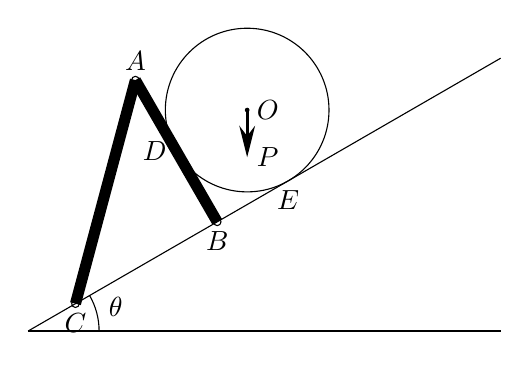
\begin{tikzpicture}[scale=0.6]
        \draw (0,0) -- (10,0);
        \draw (0,0) -- (10,10/1.732);
        \draw (1.5,0) arc (0:30:1.5);
        \coordinate [label=right:$\theta$] (theta) at (1.5,0.5);
        \coordinate [label=below:$C$] (C) at (1,1/1.732);
        \draw (C) circle (0.08);
        \coordinate [label=below:$B$] (B) at (4,4/1.732);
        \draw (B) circle (0.08);
        \coordinate [label=above:$A$] (A) at (4-3/1.732,4/1.732+3);
        \draw (A) circle (0.08);
        \coordinate [label=left:$D$] (D) at (4-1.5/1.732,4/1.732+1.5);
        \coordinate [label=below:$E$] (E) at (5.5,5.5/1.732);
        \coordinate [label=right:$O$] (O) at (5.5-1.5/1.732,5.5/1.732+1.5);
        \coordinate [label=right:$P$] (P) at (5.5-1.5/1.732,5.5/1.732+0.5);
        \fill (O) circle (0.05);
        \draw (O) circle (3/1.732);
        % \draw (D) circle (0.08);
        \draw[line width=4pt] (C) -- (A);
        \draw[line width=4pt] (B) -- (A);
        \draw[\arrow, line width=1pt] (O) -- (P);
        \end{tikzpicture}
    \]
    \\


    \textbf{Solution}
    \\

    \textbf{Part One}

    取圆柱为分离体,\(D\),\(E\)处为光滑接触,圆柱受主动力\(P\),约束力\(F_ND\)及\(F_NE\)作用,
    汇交于圆柱中心\(O\)点,受力图:

    \[
    \begin{tikzpicture}[scale=0.6]
        \draw (0,0) -- (10,0);
        \coordinate [label=right:$x$] (x) at (10,10/1.732);
        \coordinate [label=right:$y$] (y) at (4-4/1.732,4/1.732+4);
        \draw[->, dashed] (0,0) -- (x);
        \draw[->, dashed] (4,4/1.732) -- (y);
        \draw[dashed] (D) -- (7-1.5/1.732,7/1.732+1.5);
        \draw[dashed] (E) -- (5.5-3/1.732,5.5/1.732+3);
        \coordinate [label=right:$D$] (D) at (4-1.5/1.732,4/1.732+1.5);
        \coordinate [label=left:$F_{ND}$] (F_ND) at (2.5-1.5/1.732,2.5/1.732+1.5);
        \coordinate [label=below:$E$] (E) at (5.5,5.5/1.732);
        \coordinate [label=below:$F_{NE}$] (F_NE) at (5.5+1.5/1.732,5.5/1.732-1.5);
        \coordinate [label=right:$O$] (O) at (5.5-1.5/1.732,5.5/1.732+1.5);
        \coordinate [label=right:$P$] (P) at (5.5-1.5/1.732,5.5/1.732+0.5);
        \fill (O) circle (0.05);
        \draw (O) circle (3/1.732);
        \draw[\arrow, line width=1pt] (O) -- (P);
        \draw[\arrow, line width=1pt] (F_ND) -- (D);
        \draw[\arrow, line width=1pt] (F_NE) -- (E);
    \end{tikzpicture}
    \]

    取如图所示坐标轴,由平衡条件\(\sum F_x = 0\),即

    \[
    F_{ND} - P \sin \theta = 0
    \]

    解得

    \[
    F_{ND} = 25 {\rm kN}
    \]

    \textbf{Part Two}

    \(AC\)为二力构件,受力图:

    \[
    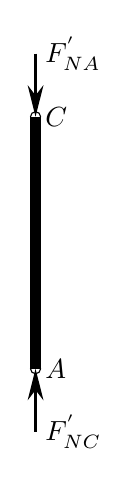
\begin{tikzpicture}[scale=0.8]
        \coordinate [label=right:$C$] (C) at (0,4);
        \draw (C) circle (0.08);
        \coordinate [label=right:$A$] (A) at (0,0);
        \draw (A) circle (0.08);
        \draw[line width=4pt] (A) -- (C);
        \coordinate [label=right:$F_{NA}^{'}$] (F_NA_) at (0,5);
        \coordinate [label=right:$F_{NC}^{'}$] (F_NC_) at (0,-1);
        \draw[\arrow, line width=1pt] (F_NA_) -- (C);
        \draw[\arrow, line width=1pt] (F_NC_) -- (A);
    \end{tikzpicture}
    \]

    \textbf{Part Three}

    取构件\(AB\)为分离体,$F_{ND}^{'}$与$F_{NA}$的作用线交于\(G\)点,由\textbf{三力平衡汇交},
    \(B\)铰约束力一定过\(G\)点,受力图:

    \[
        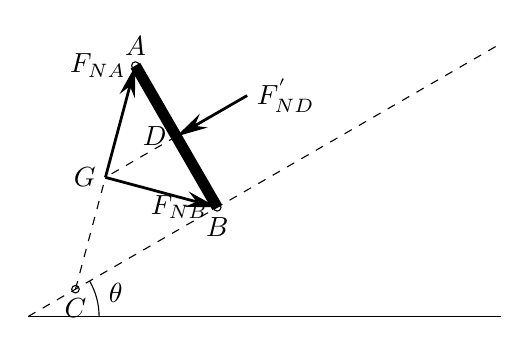
\begin{tikzpicture}[scale=0.6]
        \draw (0,0) -- (10,0);
        \draw[dashed] (0,0) -- (10,10/1.732);
        \draw (1.5,0) arc (0:30:1.5);
        \coordinate [label=right:$\theta$] (theta) at (1.5,0.5);
        \coordinate [label=below:$C$] (C) at (1,1/1.732);
        \draw (C) circle (0.08);
        \coordinate [label=below:$B$] (B) at (4,4/1.732);
        \draw (B) circle (0.08);
        \coordinate [label=above:$A$] (A) at (4-3/1.732,4/1.732+3);
        \draw (A) circle (0.08);
        \coordinate [label=left:$G$] (G) at (2.5-1.5/1.732,2.5/1.732+1.5);
        \coordinate [label=left:$D$] (D) at (4-1.5/1.732,4/1.732+1.5);
        \coordinate [label=right:$F_{ND}^{'}$] (F_ND_) at (5.5-1.5/1.732,5.5/1.732+1.5);
        \coordinate [label=left:$F_{NA}$] (F_NA) at (4-3/1.732,4/1.732+3);
        \coordinate [label=left:$F_{NB}$] (F_NB) at (4,4/1.732);
        \draw[\arrow, line width=1pt] (G) -- (F_NA);
        \draw[\arrow, line width=1pt] (G) -- (F_NB);
        \draw[\arrow, line width=1pt] (F_ND_) -- (D);
        \draw[dashed] (C) -- (A);
        \draw[line width=4pt] (B) -- (A);
        \draw[dashed] (D) -- (G);
        \end{tikzpicture}
    \]

    由\(\sum F_y = 0\),即

    \[
    F_{NA}\sin 45\degree - F_{NB} \sin 45\degree = 0
    \]

    解得

    \[
    F_{NA} = F_{NB}
    \]

    由\(\sum F_x = 0\),即

    \[
    F_{NA}\cos 45\degree + F_{NB}\cos 45\degree - F_{ND}^{'} = 0
    \]

    解得

    \[
    F_{NA} = F_{NB} = \frac{1}{\sqrt{2}} F_{ND}^{'} = 17.68 {\rm kN}
    \]


\end{homeworkProblem}

\pagebreak

\begin{homeworkProblem}
    如图所示机构自重不计,圆轮上的销子\textit{A}放置在摇杆\textit{BC}上的光滑导槽内。
    圆轮上作用有一力偶$M_1$,其力偶矩为$2 {\rm kN \cdot m}$,$OA = r = 0.5 {\rm m}$,
    图示位置时$OA$与$OB$垂直,$\theta = 30^{\circ}$,且系统平衡。求作用在摇杆上的力偶矩
    $M_2$及铰链\textit{O},\textit{B}处的约束力。

    \begin{figure}[htbp]
        \centering
        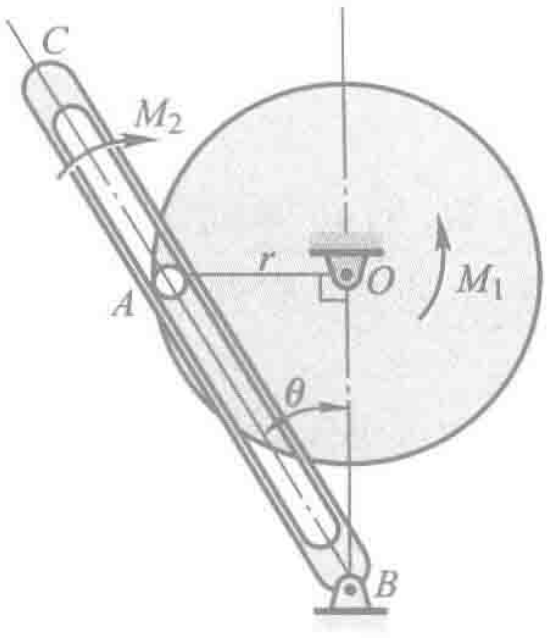
\includegraphics[scale=0.3]{images/pic1.png}
        % \caption{}
        \label{pic1}
    \end{figure}

    \textbf{Solution}
    \\

    \textbf{Part One}

    取圆轮为研究对象。

    注意到圆轮受到$A$点的光滑接触约束,因此约束力$F_A$是垂直于摇杆的。

    已知圆轮受到力偶$M_1$和力$F_A$、$F_O$的作用。因为\textbf{力偶只能由力偶来平衡},
    所以力$F_A$和$F_O$大小相等、方向相反。


    \[
    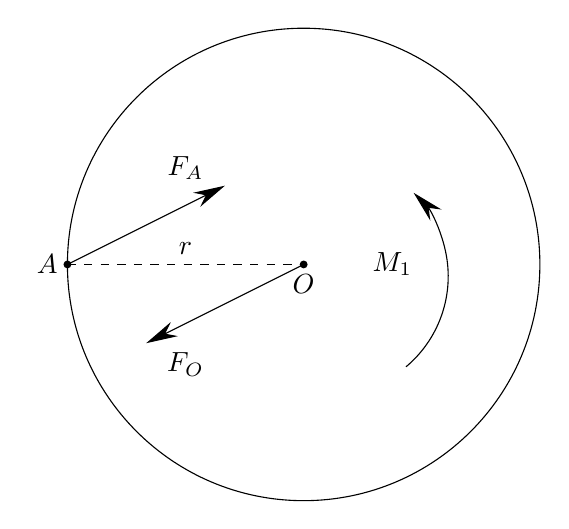
\begin{tikzpicture}
    \coordinate [label=below:$F_A$] (F_A) at (-1.5,1.5);
    \coordinate [label=below:$F_O$] (F_O) at (-1.5,-1);
    \draw (0,0) circle (3);
    \coordinate [label=left:$A$] (A) at (-3,0);
    \fill (-3,0) circle (0.05);
    \coordinate [label=below:$O$] (O) at (0,0);
    \fill (0,0) circle (0.05);
    \draw[\arrow] (A) -- (-1, 1);
    \draw[\arrow] (O) -- (-2, -1);
    \coordinate [label=left:$M_1$] (M_1) at (1.5,0);
    \draw[dashed] (A) -- (O);
    \coordinate [label=above:$r$] (r) at (-1.5,0);
    \draw[\arrow] (1.3,-1.3) arc (-50:45:1.5);
    \end{tikzpicture}
    \]

    由平衡条件$\sum M_i = 0$:
    
    \[
        M_1 - F_A r \sin\theta = 0
    \]

    解得:
    \[
        F_A = \frac{M_1}{r \sin 30^{\circ}} = 8 {\rm kN}
    \]


    \textbf{Part Two}

    取摇杆为研究对象,分析受力。

    $B$点是光滑铰链约束,因为\textbf{力偶只能由力偶来平衡},所以力$F_B$和$F_A^{'}$大小相等、
    方向相反。

    \[
        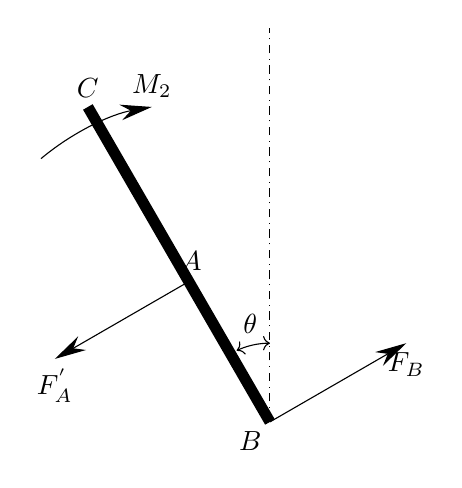
\begin{tikzpicture}
        \draw[dash dot] (0,0) -- (0,5);
        \draw[line width=4pt] (0,0) -- (-4/1.73,4);
        \coordinate [label=above:$C$] (C) at (-4/1.73,4);
        \draw[<->] (0,1) arc (90:115:1);
        \coordinate [label=above:$\theta$] (theta) at (-0.25,1);
        \draw[{Stealth[length=4mm,width=2mm]}-] (-1.5,4) arc (100:130:3);
        \coordinate [label=above:$M_2$] (M_2) at (-1.5,4);
        \coordinate [label=below:$B$] (B) at (-0.25,0);
        \coordinate [label=above:$A$] (A) at (-1,1.8);
        \coordinate [label=below:$F_A^{'}$] (F_A_) at (-1-1.732,0.8);
        \draw[\arrow] (A) -- (F_A_);
        \draw[\arrow] (0,0) -- (1.732, 1);
        \coordinate [label=below:$F_B$] (F_B) at (1.732, 1);
        \end{tikzpicture}
    \]

    由平衡条件$\sum M_i = 0$:

    \[
        -M_2 + F_A^{'} \frac{r}{\sin \theta} = 0
    \]

    解得:
    \[
        M_2 = 8 {\rm kN \cdot m}
    \]
    \[
    F_O = F_B = F_A = 8 {\rm kN}
    \]

\end{homeworkProblem}

\pagebreak

\begin{homeworkProblem}

    两齿轮的节圆半径分别为\(r_1\)、\(r_2\),作用于轮\uppercase\expandafter{\romannumeral1}上的主动力偶的力偶矩为\(M_1\),
    齿轮压力角为\(\theta\),不计两齿轮的重量。求是两齿轮维持匀速转动时齿轮\uppercase\expandafter{\romannumeral2}
    的阻力偶之矩\(M_2\)与轴承\(O_1\),\(O_2\)的约束力大小和方向。

    \[
        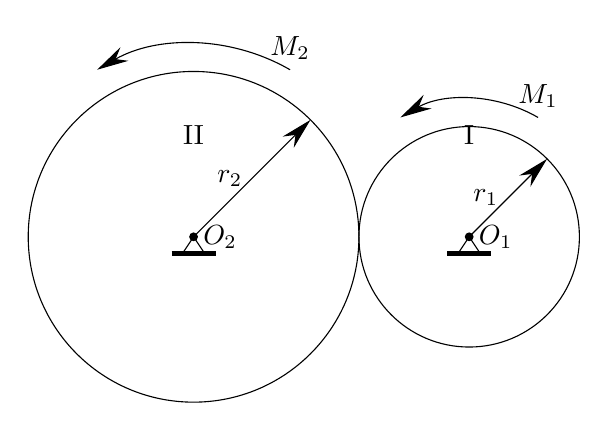
\begin{tikzpicture}[scale=0.7]
        \coordinate[label=right:$O_1$] (O_1) at (2,0);
        \coordinate[label=right:$O_2$] (O_2) at (-3,0);
        \draw (O_1) circle (2);
        \draw (O_2) circle (3);
        \fill (O_1) circle (0.08);
        \fill (O_2) circle (0.08);
        \draw (O_1) -- (1.8,-0.3);
        \draw (O_1) -- (2.2,-0.3);
        \draw (O_2) -- (-3.2,-0.3);
        \draw (O_2) -- (-2.8,-0.3);
        \draw[line width=2pt] (1.6,-0.3) -- (2.4,-0.3);
        \draw[line width=2pt] (-3.4,-0.3) -- (-2.6,-0.3);
        \coordinate [label=above:\uppercase\expandafter{\romannumeral1}] (I) at (2,1.5);
        \coordinate [label=above:\uppercase\expandafter{\romannumeral2}] (II) at (-3,1.5);
        \draw[\arrow] (O_1) -- (2+2/1.414,2/1.414);
        \draw[\arrow] (O_2) -- (-3+3/1.414,3/1.414);
        \coordinate [label=left:$r_1$] (r_1) at (2+1/1.414,1/1.414);
        \coordinate [label=left:$r_2$] (r_2) at (-3+1.5/1.414,1.5/1.414);
        \coordinate [label=above:$M_1$] (M_1) at (3.25,1.25*1.732);
        \coordinate [label=above:$M_2$] (M_2) at (-1.25,1.75*1.732);
        \draw[\arrow] (M_1) arc (60:120:2.5);
        \draw[\arrow] (M_2) arc (60:120:3.5);
        \end{tikzpicture}
    \]
    \\

    \textbf{Solution}
    \\

    {\color{BrickRed} \textbf{压力角}是指不计算摩擦力的情况下,受力方向和运动方向所夹的锐角。}
    \\

    \textbf{Part One}

    对轮\uppercase\expandafter{\romannumeral1} 进行受力分析:

    \[
        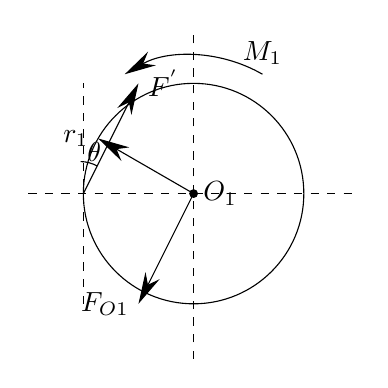
\begin{tikzpicture}[scale=0.7]
        \coordinate[label=right:$O_1$] (O_1) at (2,0);
        \draw[dashed] (-1,0) -- (5,0);
        \draw[dashed] (2,-3) -- (2,3);
        \draw (O_1) circle (2);
        \fill (O_1) circle (0.08);
        \coordinate [label=left:$r_1$] (r_1) at (2-1.732,1);
        \draw[\arrow] (O_1) -- (r_1);
        \coordinate [label=above:$M_1$] (M_1) at (3.25,1.25*1.732);
        \draw[\arrow] (M_1) arc (60:120:2.5);
        \coordinate [label=right:$F^{'}$] (F_) at (1,2);
        \coordinate [label=left:$F_{O1}$] (F_O1) at (1,-2);
        \draw[\arrow] (0,0) -- (F_);
        \draw[\arrow] (2,0) -- (F_O1);
        \draw[dashed] (0,-2) -- (0,2);
        \draw (0.25,0.5) arc (60:90:0.6);
        \coordinate [label=above:$\theta$] (theta) at (0.2,0.4);
        \end{tikzpicture}
    \]

    由平衡条件$\sum M_i = 0$:

    \[
    M_1 - F_{O1} r_1 \cos \theta = 0
    \]

    解得

    \[
        F_{O1} = \frac{M_1}{r_1 \cos \theta}
    \]

    (方向如图)

    \textbf{Part Two}

    同理可得轴承\(O_2\)约束力

    \[
        F_{O2} = \frac{M_2}{r_2 \cos \theta}
    \]

    \[
        M_{2} = \frac{r_2}{r_1} M_1
    \]

\end{homeworkProblem}

\pagebreak

\begin{homeworkProblem}

    如图所示,梯形的水坝可以看作由左边的矩形部分和右边的三角形部分组合而成。
    左边部分的重力\(P_{1} = 450 \mathrm{kN}\),右边部分的重力\(P_{2} = 200 \mathrm{kN}\),
    上游水库给水坝的压力\(F_{1} = 300 \mathrm{kN}\),下游河流给水坝的压力\(F_{2} = 70 \mathrm{kN}\)。
    各力的作用方向、位置如图所示。
    
    \[
        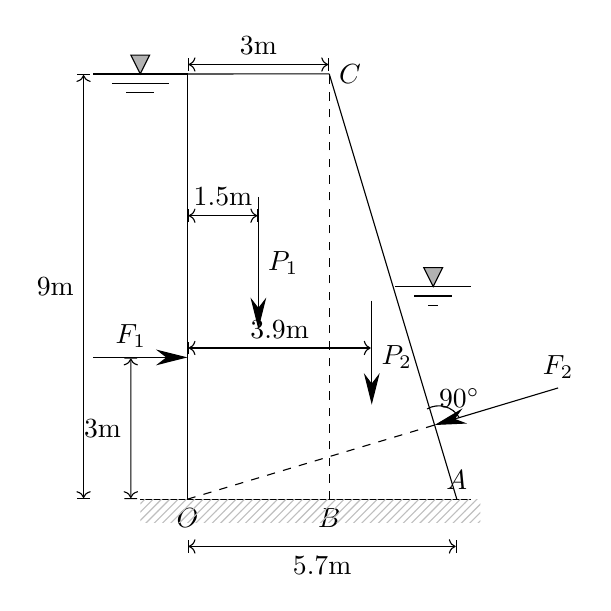
\begin{tikzpicture}[scale=0.6]
        \coordinate[label=below:$O$] (O) at (0,0);
        \coordinate[label=above:$A$] (A) at (5.7,0);
        \coordinate[label=below:$B$] (B) at (3,0);
        \coordinate[label=right:$C$] (C) at (3,9);
        \draw (-1,0) -- (6,0);
        \fill[pattern=north east lines, pattern color=gray!50] (-1,0) rectangle (6.2,-0.5);
        \draw[dashed] (B) -- (C);
        \draw (O) -- (0,9);
        \draw (C) -- (0,9);
        \draw (C) -- (A);
        % 右侧河流
        \draw (4.4,4.5) -- (6,4.5);
        \draw (4.8,4.3) -- (5.6,4.3);
        \draw (5.1,4.1) -- (5.3,4.1);
        \draw[fill=black!30] (5.2,4.5) -- (5,4.9) -- (5.4,4.9) -- cycle;
        % 左侧水库
        \draw (-2,9) -- (0,9);
        \draw (-1.6,8.8) -- (-0.4,8.8);
        \draw (-1.3,8.6) -- (-0.7,8.6);
        \draw[fill=black!30] (-1,9) -- (-1.2,9.4) -- (-0.8,9.4) -- cycle;
        % 尺寸标注
        \draw[|<->|] (-2.2,0) -- (-2.2,9) node[midway, left] {$\mathrm{9 m}$};
        \coordinate[label=above:$F_1$] (F_1) at (-1.2,3);  % 力标注
        \draw[|<->|] (-1.2,0) -- (F_1) node[midway, left] {$\mathrm{3 m}$};
        \draw[|<->|] (0,9.2) -- (3,9.2) node[midway, above] {$\mathrm{3 m}$};
        \draw[|<->|] (0,6) -- (1.5,6) node[midway, above] {$\mathrm{1.5 m}$};
        \draw[|<->|] (0,3.2) -- (3.9,3.2) node[midway, above] {$\mathrm{3.9 m}$};
        \draw[|<->|] (0,-1) -- (5.7,-1) node[midway, below] {$\mathrm{5.7 m}$};
        % 力标注
        \coordinate[label=above:$F_2$] (F_2) at (7.8435,2.3535);
        \draw[dashed] (O) -- (5.229,1.569);
        \draw[\arrow] (F_2) -- (5.229,1.569);
        \coordinate[label=right:$P_1$] (P_1) at (1.5,5);
        \draw[\arrow] (1.5,6.4) -- (1.5,3.6);
        \coordinate[label=right:$P_2$] (P_2) at (3.9,3);
        \draw[\arrow] (3.9,4.2) -- (3.9,2);
        \draw[\arrow] (-2,3) -- (0,3);
        % 垂直符号
        \draw (5.7519,1.7259) arc (30:120:0.5);
        \coordinate[label=above:$ 90 \degree $] (vertical) at (5.7519,1.7259);
        \end{tikzpicture}
    \]

    求

    \begin{enumerate}
        \item 力系的合力\(F_{R}\)
        \item 合力与\(OA\)的交点到点\(O\)的距离\(x\)
        \item 合力的作用线方程
    \end{enumerate}

    \textbf{Solution}
    \\

    \textbf{Part One}

    建立如图所示的坐标系,向\(O\)点简化,求主矢和主矩。

    \[
        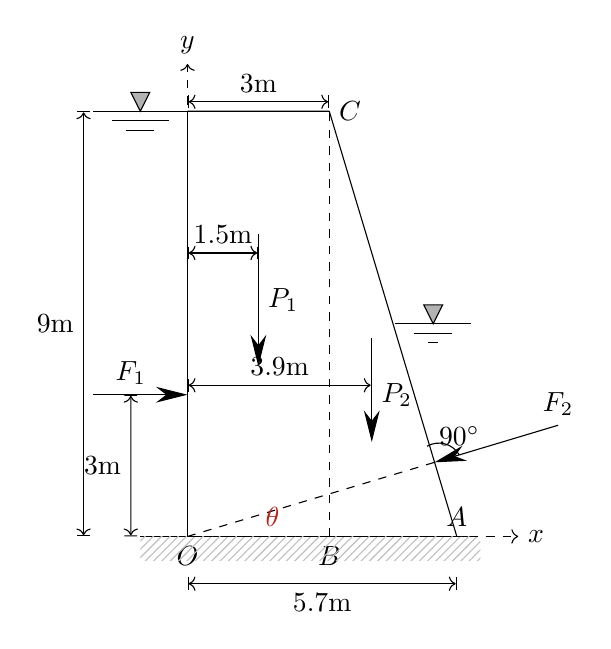
\begin{tikzpicture}[scale=0.6]
        \coordinate[label=below:$O$] (O) at (0,0);
        \coordinate[label=above:$A$] (A) at (5.7,0);
        \coordinate[label=below:$B$] (B) at (3,0);
        \coordinate[label=right:$C$] (C) at (3,9);
        % 地面阴影
        \draw (-1,0) -- (6,0);
        \fill[pattern=north east lines, pattern color=gray!50] (-1,0) rectangle (6.2,-0.5);
        \draw[dashed] (B) -- (C);
        \draw (O) -- (0,9);
        \draw (C) -- (0,9);
        \draw (C) -- (A);
        % 右侧河流
        \draw (4.4,4.5) -- (6,4.5);
        \draw (4.8,4.3) -- (5.6,4.3);
        \draw (5.1,4.1) -- (5.3,4.1);
        \draw[fill=black!30] (5.2,4.5) -- (5,4.9) -- (5.4,4.9) -- cycle;
        % 左侧水库
        \draw (-2,9) -- (0,9);
        \draw (-1.6,8.8) -- (-0.4,8.8);
        \draw (-1.3,8.6) -- (-0.7,8.6);
        \draw[fill=black!30] (-1,9) -- (-1.2,9.4) -- (-0.8,9.4) -- cycle;
        % 尺寸标注
        \draw[|<->|] (-2.2,0) -- (-2.2,9) node[midway, left] {$\mathrm{9 m}$};
        \coordinate[label=above:$F_1$] (F_1) at (-1.2,3);  % 力标注
        \draw[|<->|] (-1.2,0) -- (F_1) node[midway, left] {$\mathrm{3 m}$};
        \draw[|<->|] (0,9.2) -- (3,9.2) node[midway, above] {$\mathrm{3 m}$};
        \draw[|<->|] (0,6) -- (1.5,6) node[midway, above] {$\mathrm{1.5 m}$};
        \draw[|<->|] (0,3.2) -- (3.9,3.2) node[midway, above] {$\mathrm{3.9 m}$};
        \draw[|<->|] (0,-1) -- (5.7,-1) node[midway, below] {$\mathrm{5.7 m}$};
        % 力标注
        \coordinate[label=above:$F_2$] (F_2) at (7.8435,2.3535);
        \draw[dashed] (O) -- (5.229,1.569);
        \draw[\arrow] (F_2) -- (5.229,1.569);
        \coordinate[label=right:$P_1$] (P_1) at (1.5,5);
        \draw[\arrow] (1.5,6.4) -- (1.5,3.6);
        \coordinate[label=right:$P_2$] (P_2) at (3.9,3);
        \draw[\arrow] (3.9,4.2) -- (3.9,2);
        \draw[\arrow] (-2,3) -- (0,3);
        % 垂直符号
        \draw (5.7519,1.7259) arc (30:120:0.5);
        \coordinate[label=above:$ 90 \degree $] (vertical) at (5.7519,1.7259);
        % 建立坐标系
        \coordinate[label=right:$x$] (x) at (7,0);
        \coordinate[label=above:$y$] (y) at (0,10);
        \draw[->,dashed] (O) -- (x);
        \draw[->,dashed] (O) -- (y);
        % 夹角
        \coordinate[label={[BrickRed]above:$\theta$}] (theta) at (1.8,0);
        \end{tikzpicture}
    \]

    先计算主矢。注意到只有力$F_2$的方向较为特殊,记$F_2$与水平方向夹角为\(\theta\),则

    \[
    \theta = \angle ACB = \arctan \frac{AB}{BC} = \arctan 0.3 \approx 16.7 \degree 
    \]

    于是

    \[
    F_{Rx}^{'} = \sum F_{ix} = F_{1} - F_{2} \cos \theta \approx 232.9 \mathrm{kN}
    \]

    \[
    F_{Ry}^{'} = \sum F_{iy} = -P_{1} -P_{2} - F_{2} \sin \theta \approx -670.1 \mathrm{kN}
    \]

    所以

    \[
    F_{R}^{'} = \sqrt{\left(\sum F_{ix}\right)^2 + \left(\sum F_{iy}\right)^2} \approx 709.1 \mathrm{kN}
    \]

    于是\(F_{R}^{'}\)的方向余弦

    \[
    \cos\left( \vec{F_{R}^{'}}, \vec{i}\right) = \frac{\sum F_{ix}}{F_{R}^{'}} \approx 0.3283
    \]


    \[
    \cos\left( \vec{F_{R}^{'}}, \vec{j}\right) = \frac{\sum F_{iy}}{F_{R}^{'}} \approx -0.9446
    \]

    所以主矢与\(x\)轴正向夹角

    \[
    \alpha \approx 70.84 \degree
    \]

    主矢与\(y\)轴负向夹角

    \[
    \beta \approx 19.16 \degree
    \]

    在图中表示:

    \[
        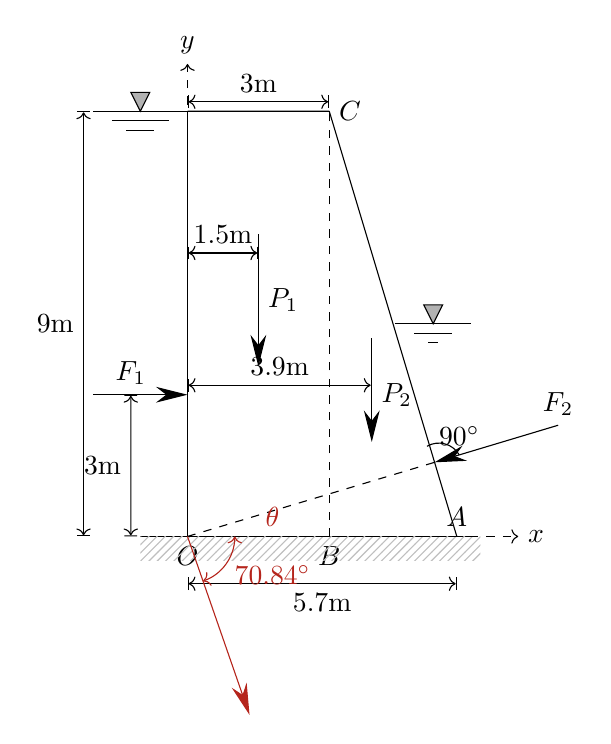
\begin{tikzpicture}[scale=0.6]
        \coordinate[label=below:$O$] (O) at (0,0);
        \coordinate[label=above:$A$] (A) at (5.7,0);
        \coordinate[label=below:$B$] (B) at (3,0);
        \coordinate[label=right:$C$] (C) at (3,9);
        % 地面阴影
        \draw (-1,0) -- (6,0);
        \fill[pattern=north east lines, pattern color=gray!50] (-1,0) rectangle (6.2,-0.5);
        \draw[dashed] (B) -- (C);
        \draw (O) -- (0,9);
        \draw (C) -- (0,9);
        \draw (C) -- (A);
        % 右侧河流
        \draw (4.4,4.5) -- (6,4.5);
        \draw (4.8,4.3) -- (5.6,4.3);
        \draw (5.1,4.1) -- (5.3,4.1);
        \draw[fill=black!30] (5.2,4.5) -- (5,4.9) -- (5.4,4.9) -- cycle;
        % 左侧水库
        \draw (-2,9) -- (0,9);
        \draw (-1.6,8.8) -- (-0.4,8.8);
        \draw (-1.3,8.6) -- (-0.7,8.6);
        \draw[fill=black!30] (-1,9) -- (-1.2,9.4) -- (-0.8,9.4) -- cycle;
        % 尺寸标注
        \draw[|<->|] (-2.2,0) -- (-2.2,9) node[midway, left] {$\mathrm{9 m}$};
        \coordinate[label=above:$F_1$] (F_1) at (-1.2,3);  % 力标注
        \draw[|<->|] (-1.2,0) -- (F_1) node[midway, left] {$\mathrm{3 m}$};
        \draw[|<->|] (0,9.2) -- (3,9.2) node[midway, above] {$\mathrm{3 m}$};
        \draw[|<->|] (0,6) -- (1.5,6) node[midway, above] {$\mathrm{1.5 m}$};
        \draw[|<->|] (0,3.2) -- (3.9,3.2) node[midway, above] {$\mathrm{3.9 m}$};
        \draw[|<->|] (0,-1) -- (5.7,-1) node[midway, below] {$\mathrm{5.7 m}$};
        % 力标注
        \coordinate[label=above:$F_2$] (F_2) at (7.8435,2.3535);
        \draw[dashed] (O) -- (5.229,1.569);
        \draw[\arrow] (F_2) -- (5.229,1.569);
        \coordinate[label=right:$P_1$] (P_1) at (1.5,5);
        \draw[\arrow] (1.5,6.4) -- (1.5,3.6);
        \coordinate[label=right:$P_2$] (P_2) at (3.9,3);
        \draw[\arrow] (3.9,4.2) -- (3.9,2);
        \draw[\arrow] (-2,3) -- (0,3);
        % 垂直符号
        \draw (5.7519,1.7259) arc (30:120:0.5);
        \coordinate[label=above:$ 90 \degree $] (vertical) at (5.7519,1.7259);
        % 建立坐标系
        \coordinate[label=right:$x$] (x) at (7,0);
        \coordinate[label=above:$y$] (y) at (0,10);
        \draw[->,dashed] (O) -- (x);
        \draw[->,dashed] (O) -- (y);
        % 夹角
        \coordinate[label={[BrickRed]above:$\theta$}] (theta) at (1.8,0);
        % 主矢
        \draw[\arrow,BrickRed] (O) -- (1.3128,-3.7784);
        \coordinate[label={[BrickRed]below:$70.84\degree$}] (degree) at (1.8,-0.4);
        \draw[<->,BrickRed] (1,0) arc (0:-70.84:1);
        \end{tikzpicture}
    \]

    再计算主矩:

    \[
    M_{O} = \sum M_{O} \left(\vec{F}\right) = -3\mathrm{m} \cdot F_{1} - 1.5\mathrm{m} \cdot P_{1}
    - 3.9\mathrm{m} \cdot P_{2} = -2355 \mathrm{kN \cdot m}
    \]

    \textbf{Part Two}

    向\(O\)点简化的主矢和主矩如图:

    \[
        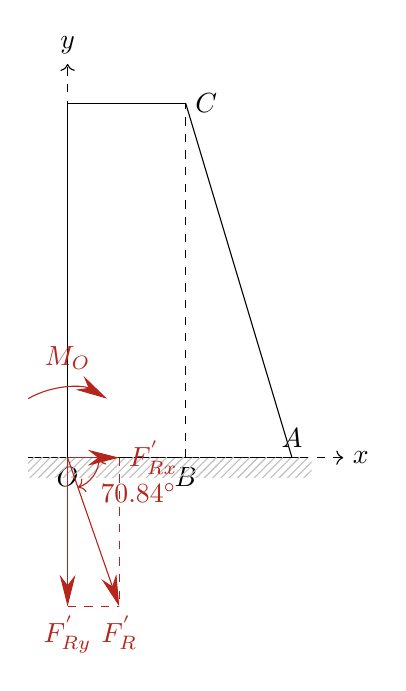
\begin{tikzpicture}[scale=0.5]
        \coordinate[label=below:$O$] (O) at (0,0);
        \coordinate[label=above:$A$] (A) at (5.7,0);
        \coordinate[label=below:$B$] (B) at (3,0);
        \coordinate[label=right:$C$] (C) at (3,9);
        % 地面阴影
        \draw (-1,0) -- (6,0);
        \fill[pattern=north east lines, pattern color=gray!50] (-1,0) rectangle (6.2,-0.5);
        \draw[dashed] (B) -- (C);
        \draw (O) -- (0,9);
        \draw (C) -- (0,9);
        \draw (C) -- (A);
        \coordinate[label=right:$x$] (x) at (7,0);
        \coordinate[label=above:$y$] (y) at (0,10);
        \draw[->,dashed] (O) -- (x);
        \draw[->,dashed] (O) -- (y);
        % 主矢
        \coordinate[label={[BrickRed]below:$F_{R}^{'}$}] (F_R_) at (1.3128,-3.7784);
        \draw[\arrow,BrickRed] (O) -- (F_R_);
        \coordinate[label={[BrickRed]below:$70.84\degree$}] (degree) at (1.8,-0.4);
        \draw[<->,BrickRed] (0.8,0) arc (0:-70.84:0.8);
        % 主矢分解
        \coordinate[label={[BrickRed]right:$F_{Rx}^{'}$}] (F_Rx_) at (1.3128,0);
        \coordinate[label={[BrickRed]below:$F_{Ry}^{'}$}] (F_Ry_) at (0,-3.7784);
        \draw[\arrow,BrickRed] (O) -- (F_Rx_);
        \draw[\arrow,BrickRed] (O) -- (F_Ry_);
        \draw[dashed,BrickRed] (F_Rx_) -- (F_R_);
        \draw[dashed,BrickRed] (F_Ry_) -- (F_R_);
        % 主矩
        \draw[\arrow,BrickRed] (-1,1.5) arc (120:60:2);
        \coordinate[label={[BrickRed]above:$M_{O}$}] (M_O) at (0,2);
        \end{tikzpicture}
    \]

    求合力及其作用线位置。合力\(F_{R}\)的大小和方向与主矢$F_{R}^{'}$相同,其作用线位置\(x\)值
    依据合力矩定理求得:

    \[
        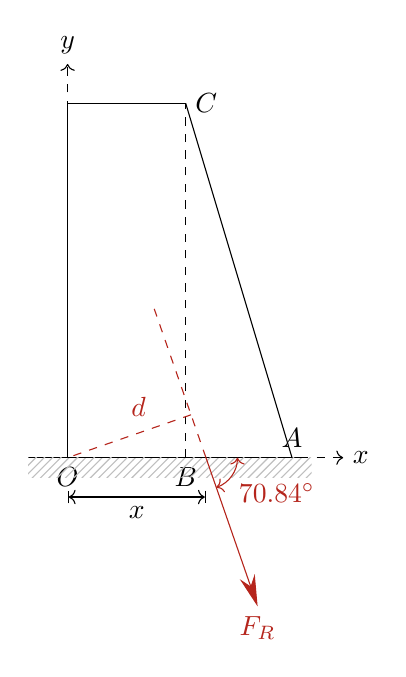
\begin{tikzpicture}[scale=0.5]
        \coordinate[label=below:$O$] (O) at (0,0);
        \coordinate[label=above:$A$] (A) at (5.7,0);
        \coordinate[label=below:$B$] (B) at (3,0);
        \coordinate[label=right:$C$] (C) at (3,9);
        % 地面阴影
        \draw (-1,0) -- (6,0);
        \fill[pattern=north east lines, pattern color=gray!50] (-1,0) rectangle (6.2,-0.5);
        \draw[dashed] (B) -- (C);
        \draw (O) -- (0,9);
        \draw (C) -- (0,9);
        \draw (C) -- (A);
        \coordinate[label=right:$x$] (x) at (7,0);
        \coordinate[label=above:$y$] (y) at (0,10);
        \draw[->,dashed] (O) -- (x);
        \draw[->,dashed] (O) -- (y);
        % 合力
        \coordinate[label={[BrickRed]below:$F_{R}$}] (F_R) at (3.514+1.3128,-3.7784);
        \draw[\arrow,BrickRed] (3.514,0) -- (F_R);
        \coordinate[label={[BrickRed]below:$70.84\degree$}] (degree) at (3.514+1.8,-0.4);
        \draw[<->,BrickRed] (3.514+0.8,0) arc (0:-70.84:0.8);
        \draw[dashed,BrickRed] (3.514,0) -- (3.514-1.3128,3.7784);
        % 标注
        \draw[|<->|] (0,-1) -- (3.514,-1) node[midway, below] {$x$};
        \draw[dashed,BrickRed] (3.13547,1.0894) -- (O);
        \coordinate[label={[BrickRed]above:$d$}] (d) at (1.8,0.8);
        \end{tikzpicture}
    \]

    由

    \[
    M_{O} = F_{R} \cdot d
    \]

    得

    \[
    d \approx 2.3197 \mathrm{m}
    \]
    
    所以

    \[
    x = \frac{d}{\sin 70.84 \degree} \approx 3.514 \mathrm{m}
    \]

    
    \textbf{Part Three}

    由于\textbf{合力可以沿其作用线移动},设合力作用线上任意一点的坐标为\(\left(x,y\right)\),将合力作用于此点,
    则合力对坐标原点的力矩的解析表达式为

    \[
    M_{O} = \sum M_{O} \left(\vec{F_{R}}\right) = x \cdot F_{Ry}^{'} - y \cdot F_{Rx}^{'}
    \]

    \[
        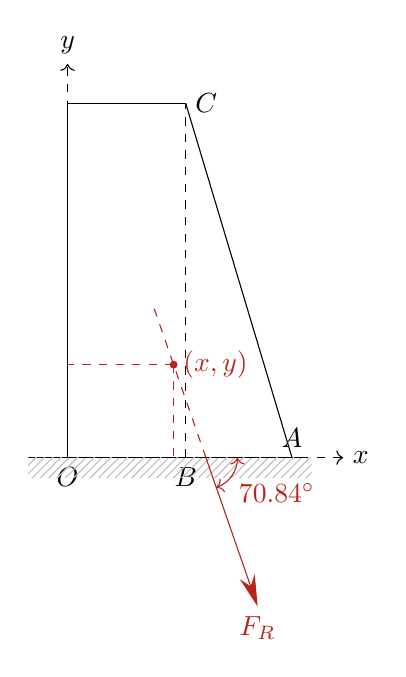
\begin{tikzpicture}[scale=0.5]
        \coordinate[label=below:$O$] (O) at (0,0);
        \coordinate[label=above:$A$] (A) at (5.7,0);
        \coordinate[label=below:$B$] (B) at (3,0);
        \coordinate[label=right:$C$] (C) at (3,9);
        % 地面阴影
        \draw (-1,0) -- (6,0);
        \fill[pattern=north east lines, pattern color=gray!50] (-1,0) rectangle (6.2,-0.5);
        \draw[dashed] (B) -- (C);
        \draw (O) -- (0,9);
        \draw (C) -- (0,9);
        \draw (C) -- (A);
        \coordinate[label=right:$x$] (x) at (7,0);
        \coordinate[label=above:$y$] (y) at (0,10);
        \draw[->,dashed] (O) -- (x);
        \draw[->,dashed] (O) -- (y);
        % 合力
        \coordinate[label={[BrickRed]below:$F_{R}$}] (F_R) at (3.514+1.3128,-3.7784);
        \draw[\arrow,BrickRed] (3.514,0) -- (F_R);
        \coordinate[label={[BrickRed]below:$70.84\degree$}] (degree) at (3.514+1.8,-0.4);
        \draw[<->,BrickRed] (3.514+0.8,0) arc (0:-70.84:0.8);
        \draw[dashed,BrickRed] (3.514,0) -- (3.514-1.3128,3.7784);
        % 标注
        \coordinate[label={[BrickRed]right:$\left(x,y\right)$}] (xy) at (3.514-1.3128/1.6,3.7784/1.6);
        \draw[dashed,BrickRed] (xy) -- (3.514-1.3128/1.6,0);
        \draw[dashed,BrickRed] (xy) -- (0,3.7784/1.6);
        \fill[BrickRed] (xy) circle (0.1);
        \end{tikzpicture}
    \]

    代入数据化简可得合力作用线方程为

    \[
    670.1x + 232.9y -2355 = 0
    \]

\end{homeworkProblem}

\pagebreak

\begin{homeworkProblem}

    如图所示不计重力的组合梁,由\(AC\)和\(CD\)在\(C\)处铰接而成。已知\(F=20 \mathrm{kN}\),
    均布载荷\(q=10 \mathrm{kN / m}\),\(M=20 \mathrm{kN \cdot m}\),\(l=1 \mathrm{m}\),
    求固定端\(A\)与滚动支架\(B\)的约束力。
    
    \[
        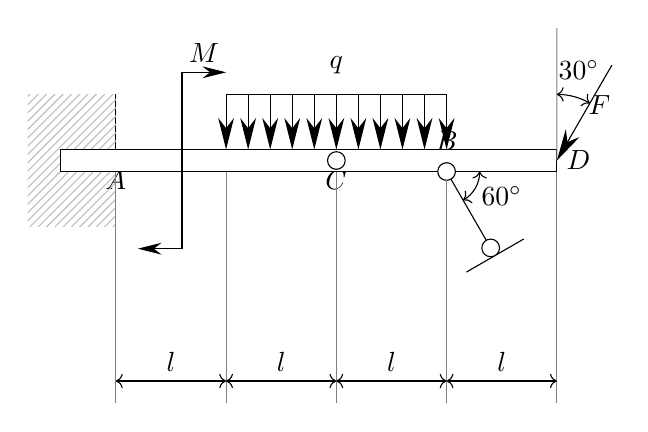
\begin{tikzpicture}[scale=1.4]
        % \coordinate[label=below:$O$] (O) at (0,0);
        \coordinate[label=below:$A$] (A) at (0,0);
        \coordinate[label=above:$B$] (B) at (3,0);
        \coordinate[label=below:$C$] (C) at (2,0);
        \coordinate[label=right:$D$] (D) at (4,0);
        \draw (0,-0.6) -- (0,0.6);
        \fill[pattern=north east lines, pattern color=gray!50] (-0.8,-0.6) rectangle (0,0.6);
        \draw[fill=white] (-0.5,-0.1) rectangle (4,0.1);
        \draw[fill=white] (C) circle (0.08);
        \draw (3+0.4,-0.1-0.4*1.732) -- (3,-0.1);
        \draw (3+0.44+0.15*1.732,-0.1-0.44*1.732+0.15) -- (3+0.44-0.15*1.732,-0.1-0.44*1.732-0.15);        \draw[fill=white] (3,-0.1) circle (0.08);
        \draw[fill=white] (3+0.4,-0.1-0.4*1.732) circle (0.08);
        % 尺寸标注
        \draw[black!50] (0,-0.1) -- (0,-2.2);
        \draw[black!50] (1,-0.1) -- (1,-2.2);
        \draw[black!50] (2,-0.1) -- (2,-2.2);
        \draw[black!50] (3,-0.1-0.08) -- (3,-2.2);
        \draw[black!50] (4,-0.1) -- (4,-2.2);
        \draw[<->] (0,-2) -- (1,-2) node[midway, above] {$l$};
        \draw[<->] (1,-2) -- (2,-2) node[midway, above] {$l$};
        \draw[<->] (2,-2) -- (3,-2) node[midway, above] {$l$};
        \draw[<->] (3,-2) -- (4,-2) node[midway, above] {$l$};
        \draw[black!50] (D) -- (4,1.2);
        \draw[<->] (4.3,0.3*1.732) arc (60:90:0.6);
        \coordinate[label=below:$30\degree$] (angelA) at (4.2,1);
        \draw[<->] (3.3,-0.1) arc (0:-60:0.3);
        \coordinate[label=below:$60\degree$] (angelB) at (3.5,-0.15);
        % 力和力矩标注
        \coordinate[label=right:$F$] (F) at (4.2,0.5);
        % \draw[dashed] (O) -- (5.229,1.569);
        \draw[\arrow] (4.5,0.5*1.732) -- (D);
        \draw[{Stealth[length=3mm,width=1.5mm]}-{Stealth[length=3mm,width=1.5mm]}] (0.2,-0.8) -- (0.6,-0.8) -- (0.6,0.8) -- (1,0.8);
        \coordinate[label=above:$M$] (M) at (0.8,0.8);
        % 载荷区间
        \draw (1,0.6) -- (3,0.6);
        \foreach \i in {0,...,10}
        {
            \draw[\arrow] (1+0.2*\i,0.6) -- (1+0.2*\i,0.1);
        }
        \coordinate[label=above:$q$] (q) at (2,0.7);
        \end{tikzpicture}
    \]
    \\

    \textbf{Solution}
    
    先画出系统所受约束力。平面任意力系,4个未知量,无法求解?\(C\)点铰链这个因素(条件)没有考虑。
    把这个因素考虑进去再分析,会发现这实质上仍是一个\textbf{静定}问题。
    \\

    \textbf{Part One}

    以\(CD\)为研究对象,画受力图。
    
    \[
        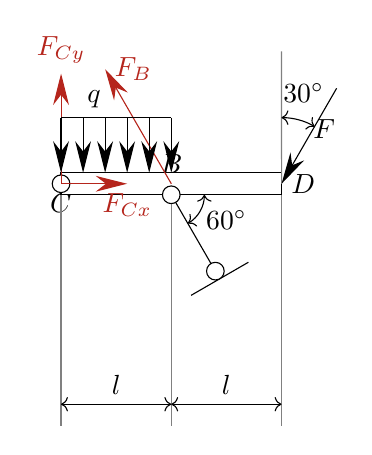
\begin{tikzpicture}[scale=1.4]
        \coordinate[label=above:$B$] (B) at (3,0);
        \coordinate[label=below:$C$] (C) at (2,0);
        \coordinate[label=right:$D$] (D) at (4,0);
        \draw[fill=white] (2,-0.1) rectangle (4,0.1);
        \draw[fill=white] (C) circle (0.08);
        \draw (3+0.4,-0.1-0.4*1.732) -- (3,-0.1);
        \draw (3+0.44+0.15*1.732,-0.1-0.44*1.732+0.15) -- (3+0.44-0.15*1.732,-0.1-0.44*1.732-0.15);        \draw[fill=white] (3,-0.1) circle (0.08);
        \draw[fill=white] (3+0.4,-0.1-0.4*1.732) circle (0.08);
        % 尺寸标注
        \draw[black!50] (2,-0.1) -- (2,-2.2);
        \draw[black!50] (3,-0.1-0.08) -- (3,-2.2);
        \draw[black!50] (4,-0.1) -- (4,-2.2);
        \draw[<->] (2,-2) -- (3,-2) node[midway, above] {$l$};
        \draw[<->] (3,-2) -- (4,-2) node[midway, above] {$l$};
        \draw[black!50] (D) -- (4,1.2);
        \draw[<->] (4.3,0.3*1.732) arc (60:90:0.6);
        \coordinate[label=below:$30\degree$] (angelA) at (4.2,1);
        \draw[<->] (3.3,-0.1) arc (0:-60:0.3);
        \coordinate[label=below:$60\degree$] (angelB) at (3.5,-0.15);
        % 力和力矩标注
        \coordinate[label=right:$F$] (F) at (4.2,0.5);
        \coordinate[label={[BrickRed]right:$F_{B}$}] (F_B) at (2.4,0.6*1.732);
        \draw[\arrow,BrickRed] (B) -- (F_B);
        \draw[\arrow] (4.5,0.5*1.732) -- (D);
        \coordinate[label={[BrickRed]below:$F_{Cx}$}] (F_Cx) at (2.6,0);
        \coordinate[label={[BrickRed]above:$F_{Cy}$}] (F_Cy) at (2,1);
        \draw[\arrow,BrickRed] (C) -- (F_Cx);
        \draw[\arrow,BrickRed] (C) -- (F_Cy);
        % 载荷区间
        \draw (2,0.6) -- (3,0.6);
        \foreach \i in {5,...,10}
        {
            \draw[\arrow] (1+0.2*\i,0.6) -- (1+0.2*\i,0.1);
        }
        \coordinate[label=above:$q$] (q) at (2.3,0.6);
        \end{tikzpicture}
    \]
    
    由\(\sum M_{C} = 0\)得

    \[
    F_{B}\sin 60\degree \cdot l - ql \cdot \frac{l}{2} - F\cos 30\degree \cdot 2l = 0
    \]

    解得

    \[
    F_{B} = 455.77 \mathrm{kN}
    \]
    \\

    \textbf{Part Two}

    取整体为研究对象,画受力图:

    \[
        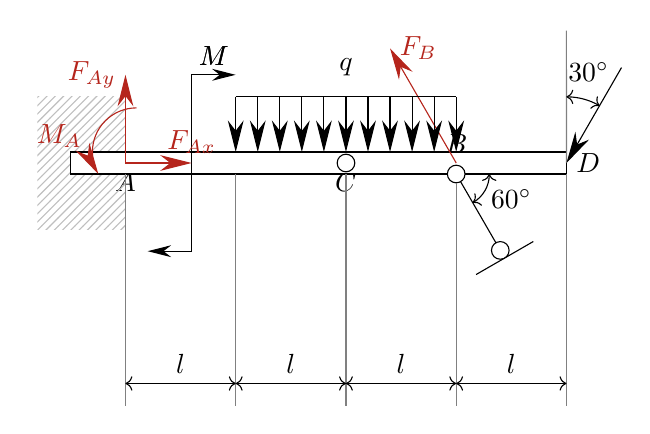
\begin{tikzpicture}[scale=1.4]
        \coordinate[label=below:$A$] (A) at (0,0);
        \coordinate[label=above:$B$] (B) at (3,0);
        \coordinate[label=below:$C$] (C) at (2,0);
        \coordinate[label=right:$D$] (D) at (4,0);
        \draw (0,-0.6) -- (0,0.6);
        \fill[pattern=north east lines, pattern color=gray!50] (-0.8,-0.6) rectangle (0,0.6);
        \draw[fill=white] (-0.5,-0.1) rectangle (4,0.1);
        \draw[fill=white] (C) circle (0.08);
        \draw (3+0.4,-0.1-0.4*1.732) -- (3,-0.1);
        \draw (3+0.44+0.15*1.732,-0.1-0.44*1.732+0.15) -- (3+0.44-0.15*1.732,-0.1-0.44*1.732-0.15);        \draw[fill=white] (3,-0.1) circle (0.08);
        \draw[fill=white] (3+0.4,-0.1-0.4*1.732) circle (0.08);
        % 尺寸标注
        \draw[black!50] (0,-0.1) -- (0,-2.2);
        \draw[black!50] (1,-0.1) -- (1,-2.2);
        \draw[black!50] (2,-0.1) -- (2,-2.2);
        \draw[black!50] (3,-0.1-0.08) -- (3,-2.2);
        \draw[black!50] (4,-0.1) -- (4,-2.2);
        \draw[<->] (0,-2) -- (1,-2) node[midway, above] {$l$};
        \draw[<->] (1,-2) -- (2,-2) node[midway, above] {$l$};
        \draw[<->] (2,-2) -- (3,-2) node[midway, above] {$l$};
        \draw[<->] (3,-2) -- (4,-2) node[midway, above] {$l$};
        \draw[black!50] (D) -- (4,1.2);
        \draw[<->] (4.3,0.3*1.732) arc (60:90:0.6);
        \coordinate[label=below:$30\degree$] (angelA) at (4.2,1);
        \draw[<->] (3.3,-0.1) arc (0:-60:0.3);
        \coordinate[label=below:$60\degree$] (angelB) at (3.5,-0.15);
        % 力和力矩标注
        \coordinate[label=above:$M$] (M) at (0.8,0.8);
        \coordinate[label={[BrickRed]right:$F_{B}$}] (F_B) at (2.4,0.6*1.732);
        \draw[\arrow,BrickRed] (B) -- (F_B);
        \draw[\arrow] (4.5,0.5*1.732) -- (D);
        \draw[{Stealth[length=3mm,width=1.5mm]}-{Stealth[length=3mm,width=1.5mm]}] (0.2,-0.8) -- (0.6,-0.8) -- (0.6,0.8) -- (1,0.8);
        \coordinate[label=above:$M$] (M) at (0.8,0.8);
        \coordinate[label={[BrickRed]left:$F_{Ay}$}] (F_Ay) at (0,0.8);
        \coordinate[label={[BrickRed]above:$F_{Ax}$}] (F_Ax) at (0.6,0);
        \coordinate[label={[BrickRed]above:$M_{A}$}] (M_A) at (-0.6,0.05);
        \draw[\arrow,BrickRed] (A) -- (F_Ax);
        \draw[\arrow,BrickRed] (A) -- (F_Ay);
        \draw[\arrow,BrickRed] (0.1,0.5) arc (90:210:0.4);
        % 载荷区间
        \draw (1,0.6) -- (3,0.6);
        \foreach \i in {0,...,10}
        {
            \draw[\arrow] (1+0.2*\i,0.6) -- (1+0.2*\i,0.1);
        }
        \coordinate[label=above:$q$] (q) at (2,0.7);
        \end{tikzpicture}
    \]

    由\(\sum F_{x} = 0\),

    \[
    F_{Ax} - F_{B}\cos60\degree - F\sin30\degree = 0
    \]

    由\(\sum F_{y} = 0\),

    \[
    F_{Ay} + F_{B}\sin60\degree - 2ql - F\cos30\degree = 0
    \]

    由\(\sum M_{A} = 0\),

    \[
    M_{A} - M - 2ql \cdot 2l + F_{B}\sin60 \degree \cdot 3l - F\cos30\degree \cdot 4l = 0
    \]

    分别解得

    \[
    M_{A} = 10.37\mathrm{kN \cdot m}, \;
    F_{Ax} = 32.89\mathrm{kN}, \;
    F_{Ay} = -2.32\mathrm{kN}
    \]

\end{homeworkProblem}

\pagebreak

\begin{homeworkProblem}

    图示结构中,已知重物重力为\(P\),\(DC=CE=AC=CB=2l\),定滑轮半径为\(R\),动滑轮半径为\(r\),
    且\(R=2r=l\),\(\theta=45\degree\)。试求\(A\)、\(E\)支座的约束力以及\(BD\)杆所受到的力。

    \[
    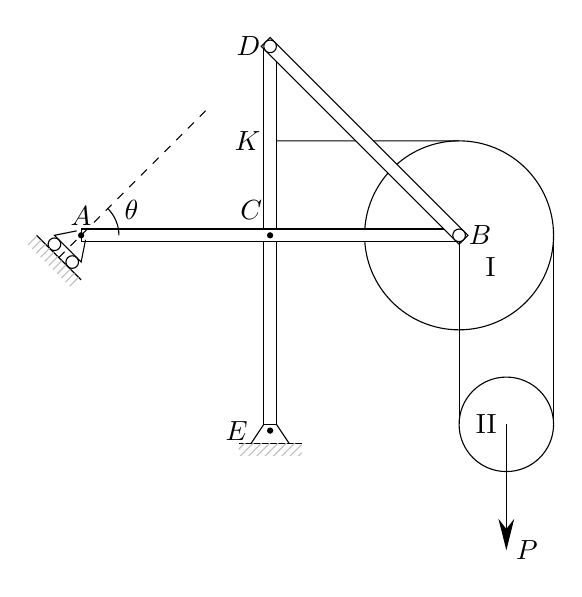
\begin{tikzpicture}[scale=0.8]
        \draw (3,0) circle (1.5);
        \coordinate[label=left:$K$] (K) at (0,1.5);
        \draw (K) -- (3,1.5);
        \coordinate[label=above:$C$] (C) at (-0.3,0.1);
        \draw[fill=white] (-0.1,-3) rectangle (0.1,3);
        \draw[fill=white] (-3,-0.1) rectangle (3,0.1);
        \fill (0,0) circle (0.05);
        \draw[fill=white,rotate=-45] (-3*1.414/2-0.1,3/1.414+0.1) rectangle (3*1.414/2+0.1,3/1.414-0.1);
        \coordinate[label=left:$E$] (E) at (-0.2,-3.1);
        \coordinate[label=left:$D$] (D) at (0,3);
        \draw[fill=white] (D) circle (0.1);
        \coordinate[label=right:$B$] (B) at (3,0);
        \draw[fill=white] (B) circle (0.1);
        \coordinate[label=above:$A$] (A) at (-3,0);
        \coordinate[label=left:\uppercase\expandafter{\romannumeral2}] (II) at (3.75,-3);
        \coordinate[label=below:\uppercase\expandafter{\romannumeral1}] (I) at (3.5,-0.2);
        \draw (II) circle (0.75);
        \draw (3,-0.1) -- (3,-3);
        \draw (4.5,0) -- (4.5,-3);
        % 重物
        \coordinate[label=right:$P$] (P) at (3.75,-5);
        \draw[\arrow] (II) -- (P);
        % 固定铰支座
        \draw (-0.3,-3.3) -- (-0.1,-3);
        \draw (0.3,-3.3) -- (0.1,-3);
        \fill (0,-3.1) circle (0.05);
        \draw (-0.5,-3.3) -- (0.5,-3.3);
        \fill[pattern=north east lines, pattern color=gray!50] (-0.5,-3.5) rectangle (0.5,-3.3);
        % 滑动铰支座
        \draw (-2.4,0) arc (0:45:0.6);
        \coordinate[label=above:$\theta$] (theta) at (-2.2,0.1);
        \draw[dashed,rotate around={45:(A)}] (-3.5,0) -- (-0.2,0);
        \draw[rotate around={45:(A)}] (-3,0.1) -- (-3.3,0.3) -- (-3.3,-0.3) -- (-3,-0.1);
        \draw[rotate around={45:(A)}] (-3.4,0.2) circle (0.1);
        \draw[rotate around={45:(A)}] (-3.4,-0.2) circle (0.1);
        \draw[rotate around={45:(A)}] (-3.5,0.5) -- (-3.5,-0.5);
        \fill[pattern=north east lines, pattern color=gray!50, rotate around={45:(A)}] (-3.5,0.5) rectangle (-3.7,-0.5);
        \fill (A) circle (0.05);
    \end{tikzpicture}
    \]

    \textbf{Solution}
    \\

    \textbf{Part One}

    取整体为研究对象,画出其受力图:

    \[
        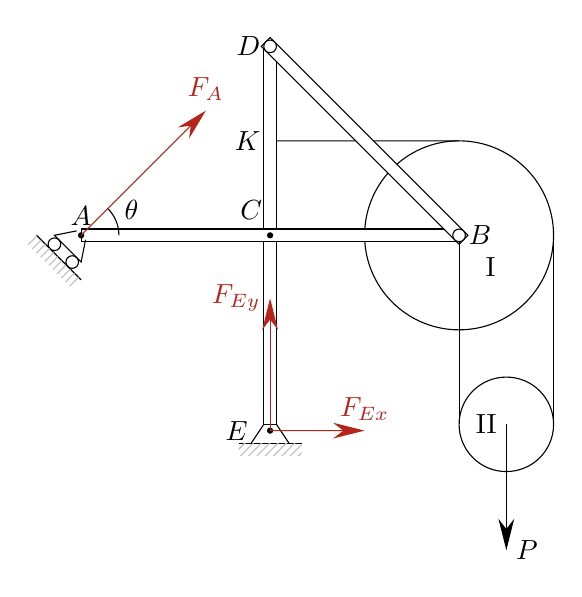
\begin{tikzpicture}[scale=0.8]
            \draw (3,0) circle (1.5);
            \coordinate[label=left:$K$] (K) at (0,1.5);
            \draw (K) -- (3,1.5);
            \coordinate[label=above:$C$] (C) at (-0.3,0.1);
            \draw[fill=white] (-0.1,-3) rectangle (0.1,3);
            \draw[fill=white] (-3,-0.1) rectangle (3,0.1);
            \fill (0,0) circle (0.05);
            \draw[fill=white,rotate=-45] (-3*1.414/2-0.1,3/1.414+0.1) rectangle (3*1.414/2+0.1,3/1.414-0.1);
            \coordinate[label=left:$E$] (E) at (-0.2,-3.1);
            \coordinate[label=left:$D$] (D) at (0,3);
            \draw[fill=white] (D) circle (0.1);
            \coordinate[label=right:$B$] (B) at (3,0);
            \draw[fill=white] (B) circle (0.1);
            \coordinate[label=above:$A$] (A) at (-3,0);
            \coordinate[label=left:\uppercase\expandafter{\romannumeral2}] (II) at (3.75,-3);
            \coordinate[label=below:\uppercase\expandafter{\romannumeral1}] (I) at (3.5,-0.2);
            \draw (II) circle (0.75);
            \draw (3,-0.1) -- (3,-3);
            \draw (4.5,0) -- (4.5,-3);
            % 重物
            \coordinate[label=right:$P$] (P) at (3.75,-5);
            \draw[\arrow] (II) -- (P);
            % 固定铰支座
            \draw (-0.3,-3.3) -- (-0.1,-3);
            \draw (0.3,-3.3) -- (0.1,-3);
            \fill (0,-3.1) circle (0.05);
            \draw (-0.5,-3.3) -- (0.5,-3.3);
            \fill[pattern=north east lines, pattern color=gray!50] (-0.5,-3.5) rectangle (0.5,-3.3);
            % 滑动铰支座
            \draw (-2.4,0) arc (0:45:0.6);
            \coordinate[label=above:$\theta$] (theta) at (-2.2,0.1);
            \draw[rotate around={45:(A)}] (-3,0.1) -- (-3.3,0.3) -- (-3.3,-0.3) -- (-3,-0.1);
            \draw[rotate around={45:(A)}] (-3.4,0.2) circle (0.1);
            \draw[rotate around={45:(A)}] (-3.4,-0.2) circle (0.1);
            \draw[rotate around={45:(A)}] (-3.5,0.5) -- (-3.5,-0.5);
            \fill[pattern=north east lines, pattern color=gray!50, rotate around={45:(A)}] (-3.5,0.5) rectangle (-3.7,-0.5);
            \fill (A) circle (0.05);
            % 受力分析
            \coordinate[rotate around={45:(A)},label={[BrickRed]above:$F_{A}$}] (F_A) at (-0.2,0);
            \draw[\arrow,rotate around={45:(A)},BrickRed] (A) -- (F_A);
            \coordinate[label={[BrickRed]left:$F_{Ey}$}] (F_Ey) at (0,-1);
            \coordinate[label={[BrickRed]above:$F_{Ex}$}] (F_Ex) at (1.5,-3.1);
            \draw[\arrow,BrickRed] (0,-3.1) -- (F_Ey);
            \draw[\arrow,BrickRed] (0,-3.1) -- (F_Ex);
        \end{tikzpicture}
        \]

        只有三个未知量,能够求解。

        由\(\sum M_{E}\left(F\right) = 0\),
    
        \[
        -2\left(F_{A} \cdot \frac{\sqrt{2}}{2} \cdot 2l\right) - P \frac{5}{2} l = 0
        \]

        由\(\sum F_{x} = 0\),

        \[
        F_{A} \cos 45 \degree + F_{Ex} = 0
        \]
    
        由\(\sum F_{y} = 0\),
    
        \[
        F_{A} \sin 45 \degree + F_{Ey} - P = 0
        \]

        分别解得

        \[
        F_{A} = -\dfrac{5\sqrt{2}}{8}P, \;
        F_{Ex} = \dfrac{5}{8} P, \;
        F_{Ey} = \dfrac{13}{8} P
        \]
        \\

        \textbf{Part Two}

        取\(DE\)杆为研究对象,画出其受力图:

        \[
            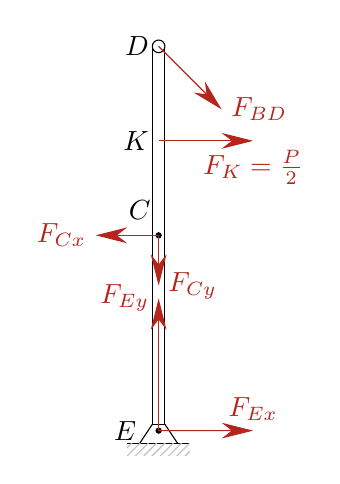
\begin{tikzpicture}[scale=0.8]
                \coordinate[label=left:$K$] (K) at (0,1.5);
                \coordinate[label=above:$C$] (C) at (-0.3,0.1);
                \draw[fill=white] (-0.1,-3) rectangle (0.1,3);
                \fill (0,0) circle (0.05);
                \coordinate[label=left:$E$] (E) at (-0.2,-3.1);
                \coordinate[label=left:$D$] (D) at (0,3);
                \draw[fill=white] (D) circle (0.1);
                \draw (-0.3,-3.3) -- (-0.1,-3);
                \draw (0.3,-3.3) -- (0.1,-3);
                \fill (0,-3.1) circle (0.05);
                \draw (-0.5,-3.3) -- (0.5,-3.3);
                \fill[pattern=north east lines, pattern color=gray!50] (-0.5,-3.5) rectangle (0.5,-3.3);
                % 受力分析
                \coordinate[label={[BrickRed]left:$F_{Ey}$}] (F_Ey) at (0,-1);
                \coordinate[label={[BrickRed]above:$F_{Ex}$}] (F_Ex) at (1.5,-3.1);
                \draw[\arrow,BrickRed] (0,-3.1) -- (F_Ey);
                \draw[\arrow,BrickRed] (0,-3.1) -- (F_Ex);
                \coordinate[label={[BrickRed]right:$F_{BD}$}] (F_BD) at (1,2);
                \draw[\arrow,BrickRed] (D) -- (F_BD);
                \coordinate[label={[BrickRed]below:$F_{K} = \frac{P}{2}$}] (F_K) at (1.5,1.5);
                \draw[\arrow,BrickRed] (K) -- (F_K);
                \coordinate[label={[BrickRed]left:$F_{Cx}$}] (F_Cx) at (-1,0);
                \draw[\arrow,BrickRed] (0,0) -- (F_Cx);
                \coordinate[label={[BrickRed]right:$F_{Cy}$}] (F_Cy) at (0,-0.8);
                \draw[\arrow,BrickRed] (0,0) -- (F_Cy);
            \end{tikzpicture}
            \]

    注意到只求\(F_{BD}\),因此由\(\sum M_{C}\left(F\right) = 0\)列平衡方程

    \[
    0 - F_{BD} \cdot \cos 45\degree \cdot 2l - F_{K} \cdot l + F_{Ex} \cdot 2l = 0
    \]

    解得

    \[
    F_{BD} = \dfrac{3\sqrt{2}}{8} P
    \]
    
\end{homeworkProblem}

\pagebreak

\begin{homeworkProblem}

    半径为\(r\)的齿轮由曲柄\(OA\)带动,沿半径为\(R\)的固定齿轮滚动。已知曲柄\(OA\)上作用一力偶矩为\(M_{1}\)的力偶,
    在齿轮\(A\)上作用一力偶矩为\(M_{2}\)的力偶,其转向如图所示。齿轮的压力角为\(\theta\),
    若不计构件的自重和摩擦,求机构平衡时\(M_{1}\)和\(M_{2}\)的关系。

    \[
    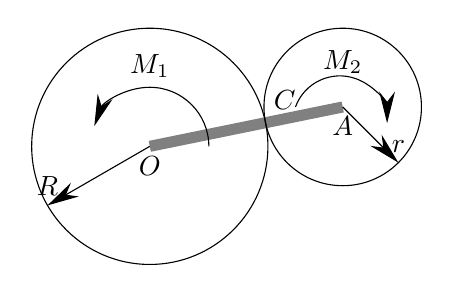
\begin{tikzpicture}[scale=0.5]
        \coordinate[label=below:$O$] (O) at (0,0);
        \coordinate[label=below:$A$] (A) at (4.9,1);
        \coordinate[label=above:$C$] (C) at (4.9*0.7,0.7);
        \draw[line width=4pt, color=black!50] (O) -- (A);
        \draw (O) circle (3);
        \draw (A) circle (2);
        \coordinate[label=above:$R$] (R) at (-1.5*1.732,-1.5);
        \draw[\arrow] (O) -- (R);
        \draw[\arrow] (1.5,0) arc (0:160:1.5);
        \draw[\arrow] (3.7,1) arc (160:0:1.2);
        \coordinate[label=above:$M_{1}$] (M_1) at (0,1.5);
        \coordinate[label=above:$M_{2}$] (M_2) at (4.9,1.6);
        \coordinate[label=above:$r$] (r) at (4.9+1.414,1-1.414);
        \draw[\arrow] (A) -- (r);
    \end{tikzpicture}
    \]

    \textbf{Solution}
    \\

    如果选整体为研究对象, 则由于支承处的约束力和齿轮啮合面\(C\)处的约束力未知,
    无法直接求出\(M_{1}\)与\(M_{2}\)之间的关系。又考虑到主动力系是平面力偶系,
    故用平面力偶系的平衡条件可方便地求得结果。

    {\color{BrickRed} 易错点:题目所说力偶\(M_{1}\)作用在曲柄\(OA\)上,而非齿轮上。
    因此,后需要对曲柄\(OA\)进行分析。}
    \\

    \textbf{Part One}

    先取齿轮\(A\)为研究对象。由于齿轮\(A\)平衡, 所以啮合力\(F\)与约束力\(F\)必组成力偶,
    其受力图下:

    \[
    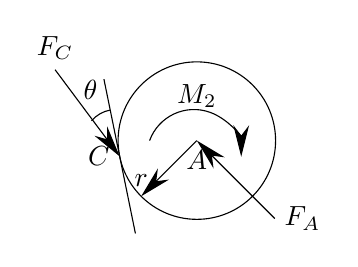
\begin{tikzpicture}[scale=0.5]
        \coordinate[label=below:$A$] (A) at (4.9,1);
        \coordinate[label=left:$C$] (C) at (4.9*0.6,0.6);
        \draw (A) circle (2);
        \draw[\arrow] (3.7,1) arc (160:0:1.2);
        \coordinate[label=above:$M_{2}$] (M_2) at (4.9,1.6);
        \draw (4.9*0.6-0.4,0.6+1.96) -- (4.9*0.6+0.4,0.6-1.96);
        \coordinate[label=above:$F_{C}$] (F_C) at (1.3,2.8);
        \draw[\arrow] (F_C) -- (C);
        \draw (4.9*0.6-0.4*0.6,0.6+1.96*0.6) arc (100:140:0.8);
        \coordinate[label=above:$\theta$] (theta) at (2.2,1.8);
        \coordinate[label=above:$r$] (r) at (4.9-1.414,1-1.414);
        \draw[\arrow] (A) -- (r);
        \coordinate[label=right:$F_{A}$] (F_A) at (4.9+1.4*1.414,1-1.4*1.414);
        \draw[\arrow] (F_A) -- (A);
    \end{tikzpicture}
    \]

    列平衡方程

    \begin{align}
    \sum{M} = 0, \;
    F_{A}r\cos\theta - M_{2} = 0 \tag{1} \label{7-1}
    \end{align}

    得

    \[
    F_{A} = \frac{M_{2}}{r\cos\theta}
    \]
    \\

    \textbf{Part Two}

    再取曲柄\(OA\)为研究对象。\(A\),\(O\)处的约束力\(F_{A}^{'}\),\(F_{O}\)组成力偶,受力图如下:

    \[
    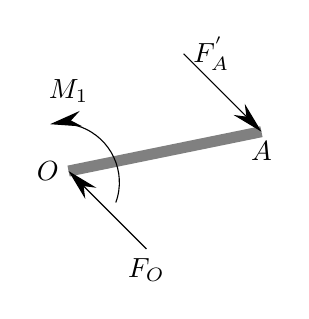
\begin{tikzpicture}[scale=0.5]
        \coordinate[label=left:$O$] (O) at (0,0);
        \coordinate[label=below:$A$] (A) at (4.9,1);
        \draw[line width=4pt, color=black!50] (O) -- (A);
        \draw[\arrow] (1.2,-0.8) arc (-20:100:1.5);
        \coordinate[label=above:$M_{1}$] (M_1) at (0,1.5);
        \coordinate[label=right:$F_{A}^{'}$] (F_A) at (4.9-1.4*1.414,1+1.4*1.414);
        \draw[\arrow] (F_A) -- (A);
        \coordinate[label=below:$F_{O}$] (F_O) at (1.4*1.414,-1.4*1.414);
        \draw[\arrow] (F_O) -- (O);
    \end{tikzpicture}
    \]

    列平衡方程如下:

    \begin{align}
    \sum{M} = 0, \;
    -F_{A}^{'}\left(r+R\right)\cos\theta + M_{1} = 0 \tag{2} \label{7-2}
    \end{align}

    得

    \[
    F_{A}^{'} = \frac{M_{1}}{\left(r+R\right)\cos\theta}
    \]

    由公式(\ref{7-1}),(\ref{7-2}),可知

    \[
    \frac{M_{2}}{r\cos\theta} = \frac{M_{1}}{\left(r+R\right)\cos\theta}
    \]
    
    则
    
    \[
    M_{2} = \frac{r}{R+r}M_{1}
    \]

    
\end{homeworkProblem}

\pagebreak

\begin{homeworkProblem}
    
    构架由不计自重的杆\(AB\)、\(AC\)和\(DF\)铰接而成,如图所示,杆\(DF\)上的销\(E\)套在杆\(AC\)的光滑槽内。
    在水平杆\(DF\)的一端作用一铅锤力\(F\),求杆\(AB\)上铰链\(A\)、\(D\)和\(B\)所受的力。

    \begin{figure}[htbp]
        \centering
        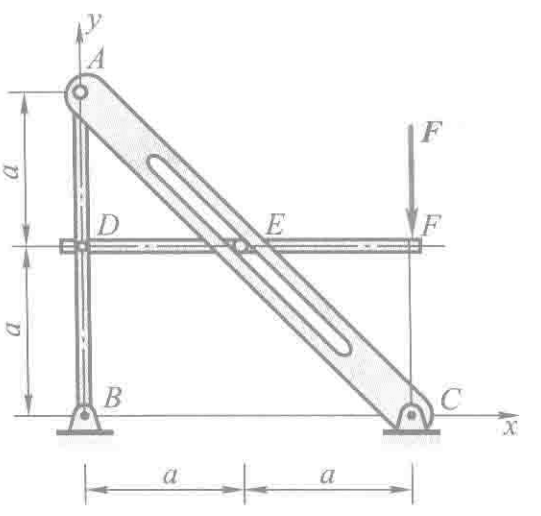
\includegraphics[scale=0.4]{images/pic2.png}
        % \caption{}
        \label{pic2}
    \end{figure}

    \textbf{Solution}
    \\

    \textbf{Part One}

    以整体为研究对象。整个系统所受外力只有\(F\)、\(F_{B}\)和\(F_{C}\),且\(F\)和\(F_{C}\)作用线均过点\(C\)。
    
    对\(C\)点取矩:

    \[
    \sum M_{C} = 0, \;
    F_{By} \cdot 2a = 0
    \]

    所以

    \[
    F_{By} = 0
    \]
    \\

    \textbf{Part Two}

    以杆\(DF\)为研究对象。因为杆\(DF\)上的销\(E\)套在杆\(AC\)的光滑槽内,所以杆\(AC\)对杆\(DF\)的力与杆\(AC\)垂直。
    受力分析如图:

    \[
    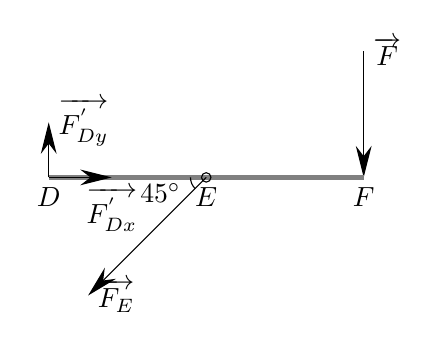
\begin{tikzpicture}
        \coordinate[label=below:$D$] (D) at (0,2);
        \coordinate[label=right:$\overrightarrow{F_{E}}$] (F_E) at (0.5,0.5);
        \coordinate[label=below:$\overrightarrow{F_{Dx}^{'}}$] (F_Dx) at (0.8,2);
        \coordinate[label=right:$\overrightarrow{F_{Dy}^{'}}$] (F_Dy) at (0,2.7);
        \coordinate[label=below:$F$] (F) at (4,2);
        \coordinate[label=below:$E$] (E) at (2,2);
        \coordinate[label=right:$\overrightarrow{F}$] (Force) at (4,3.6);
        \draw[\arrow] (Force) -- (F);
        \draw[line width=2pt,color=black!50] (D) -- (F);
        \draw (E) circle (0.06);
        \draw[\arrow] (E) -- (F_E);
        \draw[\arrow] (D) -- (F_Dx);
        \draw[\arrow] (D) -- (F_Dy);
        \draw (1.8,2) arc (180:225:0.2);
        \coordinate[label=left:$45 \degree$] (angle) at (1.8,1.8);
    \end{tikzpicture}
    \]
    
    对\(D\)点取矩,有

    \[
    F_{E} \cdot \frac{\sqrt{2}}{2} a + F \cdot 2a = 0
    \]

    解得

    \[
    F_{E} = -2\sqrt{2} F
    \]

    又由

    \[
    \sum F_{x} = 0, \;
    \sum F_{y} = 0
    \]

    有

    \[
    F_{Dx}^{'} - F_{E} \sin 45\degree = 0
    \]

    \[
    F_{Dy}^{'} - F - F_{E} \cos 45\degree = 0
    \]

    解得

    \[
    F_{Dx} = -2F, \;
    F_{Dy} = -F
    \]
    \\
    
    \textbf{Part Three}

    以杆\(AB\)为研究对象。受力分析如图:

    \[
    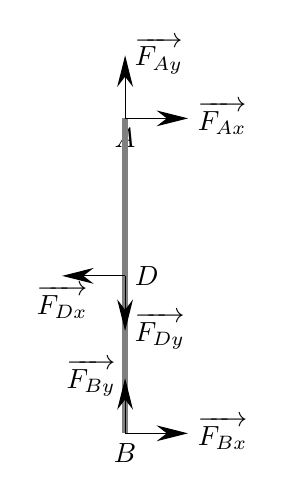
\begin{tikzpicture}
        \coordinate[label=right:$D$] (D) at (0,2);
        \coordinate[label=below:$B$] (B) at (0,0);
        \coordinate[label=below:$\overrightarrow{F_{Dx}}$] (F_Dx_) at (-0.8,2);
        \coordinate[label=right:$\overrightarrow{F_{Dy}}$] (F_Dy_) at (0,1.3);
        \coordinate[label=below:$A$] (A) at (0,4);
        \draw[line width=2pt,color=black!50] (A) -- (B);
        \coordinate[label=right:$\overrightarrow{F_{Ay}}$] (F_Ay) at (0,4.8);
        \coordinate[label=right:$\overrightarrow{F_{Ax}}$] (F_Ax) at (0.8,4);
        \coordinate[label=right:$\overrightarrow{F_{Bx}}$] (F_Bx) at (0.8,0);
        \coordinate[label=left:$\overrightarrow{F_{By}}$] (F_By) at (0,0.7);
        \draw[\arrow] (A) -- (F_Ax);
        \draw[\arrow] (A) -- (F_Ay);
        \draw[\arrow] (B) -- (F_Bx);
        \draw[\arrow] (B) -- (F_By);
        \draw[\arrow] (D) -- (F_Dx_);
        \draw[\arrow] (D) -- (F_Dy_);
    \end{tikzpicture}
    \]
    
    对\(B\)点取矩,有

    \[
    F_{Dx} \cdot a - F_{Ax} \cdot 2a = 0
    \]

    解得

    \[
    F_{Ax} = -F
    \]

    又由

    \[
    \sum F_{x} = 0, \;
    \sum F_{y} = 0
    \]

    有

    \[
    F_{Dx} + F_{Bx} + F_{Ax} = 0
    \]

    \[
    F_{Dy} - F_{By} - F_{Ay} = 0
    \]

    解得

    \[
    F_{Ay} = -F, \;
    F_{Bx} = -F
    \]

    综上所述,

    \[
    F_{Ax} = -F, \;
    F_{Ay} = -F
    \]

    \[
    F_{Bx} = -F, \;
    F_{By} = 0
    \]

    \[
    F_{Dx} = -2F, \;
    F_{Dy} = -F
    \]

\end{homeworkProblem}

\pagebreak

\end{document}
